\documentclass{article}
\usepackage{booktabs}
\usepackage{amsmath}
\usepackage{amssymb}
\usepackage[noend]{algorithmic}
\usepackage[nothing]{algorithm}
\usepackage{tikz}
\usepackage{latexsym}
\usepackage{float}
\usetikzlibrary{arrows,automata}
\providecommand{\e}[1]{\ensuremath{\times 10^{#1}}}
\renewcommand{\thealgorithm}{}
\title{CS 525: Theory of Computation\\ Midterm 1}
\author{Dustin Ingram}
\begin{document}
\maketitle
\begin{enumerate}
    \item \textbf{Solution:}
    \begin{figure}[!h]
    \centering
    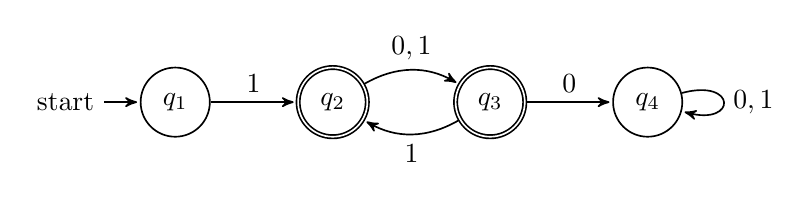
\begin{tikzpicture}[->,>=stealth',shorten >=1pt,auto,node distance=2.8cm,semithick]
      \node[state, initial]     (q1) at (0,0)  {$q_{1}$};
      \node[state, accepting]     (q2) at (2,0)  {$q_{2}$};
      \node[state, accepting]     (q3) at (4,0) {$q_{3}$};
      \node[state]     (q4) at (6,0) {$q_{4}$};

      \path (q1) edge node {$1$} (q2)
            (q2) edge[bend left] node {$0,1$} (q3)
            (q3) edge[bend left] node {$1$} (q2)
            (q3) edge node {$0$} (q4)
            (q4) edge[loop right] node {$0,1$} (q4);
    \end{tikzpicture}
    \end{figure}

    \item \textbf{Solution:}
    Using the pumping lemma, assume $L_{2}$ is regular. Let $s=b^{p+1}a^{p}$, which satisfies the condition that $|b|>|a|$. Then, if $s$ is split into $xyz$ to satisfying the conditions of the pumping lemma, by the $3^{rd}$ condition of the pumping lemma, $y$ consists only of $b$'s. Now, consider when $xy^{0}z = xz$. This decreases the number of $b$'s in $s$ such that $|b|=|a|$, breaking the condition that $|b|>|a|$, proving that $s$ cannot be a member of $L_{2}$, thereby proving that $L_{2}$ is not regular.

    \item \textbf{Solution:}
    Using the non-determinism of the PDA, the machine has two separate branches based on whether it's initial character is $a$ or $b$. Before the first character is read, the PDA pushes a \$ symbol onto the stack (to later test for an empty stack). If the first character in the string is an $a$, the PDA first reads and pushes all the $a$'s. Once it encounters a $b$, the PDA pops an $a$ off the stack. The PDA continues, pushing every $a$ and popping an $a$ every time a $b$ is read. The PDA completes successfully if it reaches the end of the string and the stack is empty (using the \$ symbol procedure). If at any point it reaches the end of the string and the stack is not empty, the PDA has failed (the end of the stack, however, may be repeatedly reached).

    \item \textbf{Solution:}
    Here, we will use the pumping lemma for context-free languages. Let $s=w\#t$ (instead of $u\#v$), where $|w|=p$ and thus since $|w|=|t|$, $|t|=p$ as well. In this case, $vxy$ must be either:
    \begin{enumerate}
        \item Wholly contained within the substring $w$;
        \item Wholly contained within the substring $t$;
        \item Split between $w$ and $t$, thus somehow containing the `\#' symbol.
    \end{enumerate}
    In 1), pumping $v$ and $y$ would result in some modification of the substring $w$, without modification to the substring $t$, therefore not guaranteeing that $w$ is a permutation of $t$. 
    In 2), the same is true as in 1), with $w$ and $t$ interchanged.
    In 3), $vxy$ must contain the `\#' symbol, which must be in $x$ (otherwise pumping would produce more than one). Again, in this case, pumping $v$ and $y$ would not guarantee that the substring $w$ is still a permutation of $t$. For example, if we take $s=aaab\#aaba$, where $p=4$, we have two possible divisions of $s$; in the case where we pump $v$ and $y$ once such that $uv^{1}xy^{1}z => uv^{2}xy^{2}z$, the following is produced:
    \begin{align*}
       \overbrace{\underbrace{aa}_{u}\underbrace{ab}_{v}}^{w}\underbrace{\#}_{x}\overbrace{\underbrace{a}_{y}\underbrace{aba}_{z}}^{t} 
       &\to \overbrace{\underbrace{aa}_{u}\underbrace{abab}_{v^{2}}}^{w}\underbrace{\#}_{x}\overbrace{\underbrace{aa}_{y^{2}}\underbrace{aba}_{z}}^{t} \\ 
       \overbrace{\underbrace{aaa}_{u}\underbrace{b}_{v}}^{w}\underbrace{\#}_{x}\overbrace{\underbrace{aa}_{y}\underbrace{ba}_{z}}^{t}
       &\to \overbrace{\underbrace{aaa}_{u}\underbrace{bb}_{v^{2}}}^{w}\underbrace{\#}_{x}\overbrace{\underbrace{aaaa}_{y^{2}}\underbrace{ba}_{z}}^{t} 
    \end{align*}
    Here it is clear that pumping $s$ does not produce a string in $L_{4}$, and thus $L_{4}$ is not context-free. 

    \item \textbf{Solution:}
    Let $M_{5}$ be a Turing machine that accepts the language of a string $s$ of 0's whose length is a prime number. Here, $M_{1}$ will use two special characters `\$' and `\#'. The machine will essentially check whether the string contains a multiple of $n \in \{2,3,4,5,\dots,|s|\}$. To begin, the machine marks the first character in the string as a `\$'. The length of this string of `\$' characters tells the machine how many 0's to skip before it marks the next character as a `\#'; in this case the length is 1 (and thus we are checking to see if it is a multiple of 2). The machine then returns to the beginning of the string, marking every other character as a `\#'. If the machine reaches the end of the string and the last character is marked as a `\#', it is not prime and thus the machine fails. However, if the machine reaches the end of the string and the last character cannot be marked as `\#', the machine returns to the beginning of the string, writing a new `\$' character after the last `\$' character, thus incrementing the factor to test. The machine terminates successfully if it marks the entire string as `\$' characters (thus, the last character is a `\$' and not a `\#' or a `0').

    \item \textbf{Solution:}
    A deterministic Turing machine must have only three states: an accept state, a reject state, and a state which is neither accept or reject. To simulate any deterministic Turing machine with more than three states, we simply must store the state transitions on the tape, such that for each possible transition, we show that it either transitions to the accepting state, the rejecting state, or remains in the `processing' state. Thus, any deterministic Turing machine can be simulated.
    \end{enumerate}
\end{document}
